\documentclass[11pt]{article}

\usepackage{amsmath, amssymb, amsthm}
\usepackage{tikz}

\theoremstyle{plain}
\newtheorem{thm}{Theorem}[section]
\newtheorem*{thm*}{Theorem}
\newtheorem{prop}[thm]{Proposition}
\newtheorem{lem}[thm]{Lemma}
\newtheorem*{lem*}{Lemma}
\newtheorem{dfn}[thm]{Definition}
\newtheorem{cor}[thm]{Corollary}
\newtheorem{claim}[thm]{Claim}
\newtheorem{conj}[thm]{Conjecture}
\newtheorem{ques}[thm]{Question}
\newtheorem*{rem}{Remark}


\oddsidemargin  0pt
\evensidemargin 0pt
\marginparwidth 40pt
\marginparsep 10pt
\topmargin 0pt
\headsep 10pt
\textheight 8.2in
\textwidth 6.4in
\renewcommand{\baselinestretch}{1.1}

\newcommand{\codeg}{\text{codeg}}
\newcommand{\BBE}{\mathbb{E}}
\newcommand{\BFP}{\mathbf{P}}
\usepackage{amsmath}
\usepackage{amsthm}
\usepackage{amssymb}
\usepackage{mathtools}
\usepackage{hyperref}
\usepackage{url}





\usepackage{graphicx}
\usepackage{caption}
\usepackage{subcaption}

\def\eQb#1\eQe{\begin{eqnarray*}#1\end{eqnarray*}}
\def\eQnb#1\eQne{\begin{eqnarray}#1\end{eqnarray}}
\providecommand{\e}[1]{\ensuremath{\times 10^{#1}}}
\providecommand{\pb}[0]{\pagebreak}
\DeclarePairedDelimiter\ceil{\lceil}{\rceil}
\DeclarePairedDelimiter\floor{\lfloor}{\rfloor}

\newcommand{\E}{\mathrm{E}}
\newcommand{\Var}{\mathrm{Var}}
\newcommand{\Cov}{\mathrm{Cov}}

\def\Qb#1\Qe{\begin{question}#1\end{question}}
\def\Sb#1\Se{\begin{solution}#1\end{solution}}


\newtheoremstyle{quest}{\topsep}{\topsep}{}{}{\bfseries}{}{ }{\thmname{#1}\thmnote{ #3}.}
\theoremstyle{quest}
\newtheorem*{definition}{Definition}
\newtheorem*{theorem}{Theorem}
\newtheorem*{lemma}{Lemma}
\newtheorem*{question}{Question}
\newtheorem*{preposition}{Preposition}
\newtheorem*{exercise}{Exercise}
\newtheorem*{challengeproblem}{Challenge Problem}
\newtheorem*{solution}{Solution}
\newtheorem*{remark}{Remark}
\usepackage{verbatimbox}
\usepackage{listings}
\usepackage{mathrsfs}
\date{}
\title{\vspace{-0.7cm}
Durrett Probability: Problems}

\author{
Youngduck Choi 
\thanks{Department of Mathematics, Courant Institute of Mathematical Sciences, 
yc1104@nyu.edu; If you find an error and want to share with me, 
you can reach me via email.
}}

\begin{document}

\maketitle

\begin{abstract}
This work contains solutions to some
exercises from Durrett's probability
text.
\end{abstract}


\section{Chapter 6: Markov Chains} \label{sec:MC}

\begin{question}[6.3.3]
\hfill
\begin{figure}[h!]
  \centering
    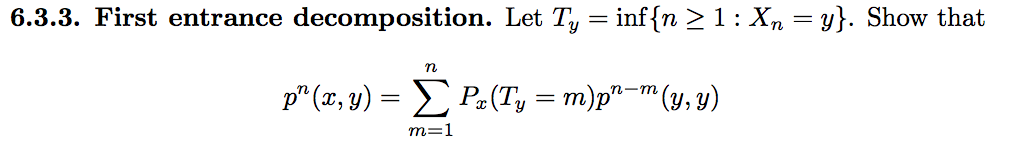
\includegraphics[width=0.7\textwidth]{d-6-3-3.png}
\end{figure}
\end{question}
\begin{solution} \hfill \\
Here we assume countable state space. Observe that
\eQnb
p^{n}(x,y) &=& P_x(X_n = y) = P_x( \bigcup_{m=1}^{n} \{ T_y = m \> ; \> X_n = y \}) 
= \sum_{m=1}^{n} P_x(T_y = m \> ; \> X_n = y) \label{eq:6.3.3.0} 
\eQne
\eQnb
P_x(T_y = m \> ; \> X_n = y) &=& E_x( 1_{\{X_n = y\}} \> ; \> T_y = m) \nonumber \\
&=& E_x(E_x(1_{\{X_n = y\}} | \mathscr{F}_m) ; T_y = m) \label{eq:6.3.3.1} \\
&=& E_x(E_x(1_{\{X_{n-m} = y \}} \circ \theta_m | \mathscr{F}_m) ; T_y = m) \nonumber \\ 
&=& E_x(E_{X_m}(1_{\{X_{n-m} = y \}} ; T_y = m) = E_x(P_y(X_{n-m} = y); T_y = m) 
\label{eq:6.3.3.2} \\ 
&=& P_x( T_y = m) P_y(X_{n-m} = y) \nonumber
\eQne
for any $1 \leq m \leq n$, where~\eqref{eq:6.3.3.1} holds by definition of conditional
expectation and~\eqref{eq:6.3.3.2} holds by Markov property.  
Therefore, combining the above result with with~\eqref{eq:6.3.3.0} gives
\eQb
p^{n}(x,y) &=& \sum_{m=1}^{n} P_x(T_y = m) P_y(X_{n-m} = y).
\eQe 

\bigskip

\noindent Here is another approach using strong Markov. We compute
\eQnb
p^{n}(x,y) &=& P_x(X_n = y) = P_x( \bigcup_{m=1}^{n} \{ T_y = m ; X_n = y \}) 
\nonumber \\ 
&=& E_x(1_{\{X_{n - T_y} = y\}} \circ \theta_{T_y} ; T_y \leq n) 
= E_x(E_x( 1_{\{X_{n - T_y} = y\}} \circ \theta_{T_y} | \mathscr{F}_{T_y}) ; T_y \leq 
n) \label{eq:6.3.3.1} \\
&=& E_x( E_{X_{T_y}}(1_{\{X_{n - T_y} = y\}} ; T_y \leq n) 
= E_x(E_y(1_{\{X_{n - T_y}\} });
T_y \leq n) \label{eq:6.3.3.2} \\
&=& \sum_{m=1}^{n} P_x(T_y = m) E_y(1_{\{ X_{n-m} = y\}}) = \sum_{m=1}^{n} P_x(
T_y = m) P^{n-m}(y,y) \nonumber 
\eQne
where~\eqref{eq:6.3.3.1} holds by definition of conditional expectation 
and~\eqref{eq:6.3.3.2} holds by the strong Markov property. \hfill $\qed$ 
\end{solution}

\newpage

\begin{question}[6.3.4]
\hfill
\begin{figure}[h!]
  \centering
    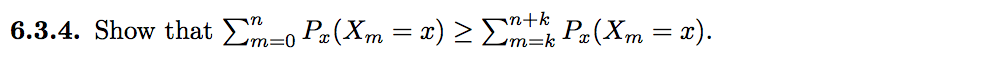
\includegraphics[width=0.7\textwidth]{d-6-3-4.png}
\end{figure}
\end{question}
\begin{solution} \hfill \\
Let $k \in \mathbb{N}$,
and $T^{k}_x = \inf\{n \geq k : X_n = x \}$. We claim that
\eQnb
P_x(X_m = x) &=& \sum_{l=k}^{m} P_x(T^{k}_x  = x)p^{m-l}(x,x) \label{eq:6.3.4.1} 
\eQne 
for any $m \geq k$. Fix $m \geq k$. Then,
\eQnb
P_x(X_m = x) &=& P_x(\bigcup_{l=k}^{m} \{ T^{k}_x = l; X_m = x\}) 
= \sum_{l=k}^{m} P_x(T^{k}_x = l ; X_m = x)\label{eq:6.3.4.2} .
\eQne
Now, we compute 
\eQnb
P_x(T^k_x = l; X_m = x ) &=& E_x(1_{\{X_m = x\}} ; T_x^{k} = l) = E_x(E_x(
1_{\{X_m = x\}} | \mathscr{F}_l) ; T_x^{k} = l) \nonumber \\
&=& E_x(E_x(1_{\{X_{m-l} = x\}} \theta_{l} | \mathscr{F}_l); T_x^{k} = l) \nonumber \\
&=& E_x(E_{X_l}(1_{\{ X_{m-l} = x\}} ; T_x^{k} = l);T_x^{k} = l) \label{eq:6.3.4.3} \\
&=& E_x(P_x(X_{m-l} x); T_x^{k} = l) = P_x(X_{m-l} = x) P_x(T_x^{k} = l) \nonumber \\ 
&=& P_x(T_x^{k} = l) p^{m-l}(x,x) \nonumber 
\eQne
for any $k \leq l \leq m$, where~\eqref{eq:6.3.4.3} holds by Markov property.
Therefore, combining the above result with~\eqref{eq:6.3.4.2},
we have proven~\eqref{eq:6.3.4.1}. Then,
\eQb
\sum_{m=k}^{n+k} P_x(X_m = x) &=& \sum_{m=k}^{n+k} \sum_{l=k}^{m} 
P_x(T^{k}_x = l)p^{m-l}(x,x) \\
&=& \sum_{l = k}^{n+k} \sum_{m = l}^{n+k} P_x(T^{k}_x = l) p^{m-l}(x,x) \\ 
&=& \sum_{m=0}^{n} p^{m}(x,x) \left( \sum_{l=k}^{d} P_x(T_x^{k} = l) \right) \\
&\leq& \sum_{m=0}^{n} p^{m}(x,x) = \sum_{m=0}^{n} P_x(X_m = x)  \\ 
\eQe 


\end{solution}

\newpage

\begin{question}[6.3.5]
\hfill
\begin{figure}[h!]
  \centering
    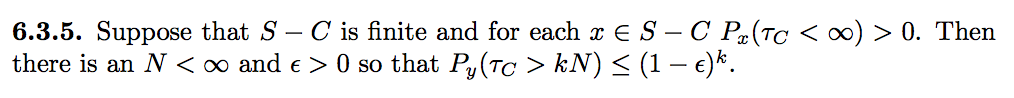
\includegraphics[width=0.7\textwidth]{d-6-3-5.png}
\end{figure}
\end{question}
\begin{solution} \hfill \\
We assume countable state space. Observe that, for any $x \in S \setminus C$,
we can choose $n(x) \in \mathbb{N}$ such that
\eQb
P_x(\tau_C \leq n) > 0.
\eQe
Otherwise, for some $x \in S \setminus C$, by continuity of probability,
\eQb
P_x(\tau_C < \infty) = \lim_{k \to \infty} P_x(\tau_C \leq k) = 0,
\eQe
which is a contradiction. Now, let
\eQb
N = \max_{z \in S \setminus C} n(x). 
\>\>\> \text{and} \>\>\>
\epsilon = \min_{z \in S \setminus C} P_z(\tau_C \leq N).
\eQe
Trivially,
\eQb
P_y(\tau_C > kN) = 0
\eQe
for any $k \in \mathbb{N}$, and $y \in C$, since $y \in C$ implies $\tau_C = 0$ 
by definition. Therefore, it suffices to show 
\eQnb
P_y(\tau_C > kN) \leq (1-\epsilon)^k \label{eq:6.3.5.1}
\eQne
for all $k \in \mathbb{N}$ and $y \in S\setminus C$. Fix $y \in S \setminus C$.
Then,
\eQb
P_y(\tau_C \leq N) &\geq&  \epsilon. 
\eQe
and hence
\eQb
P_y(\tau_C > N) \leq (1-\epsilon)
\eQe
Now, we proceed by induction to prove~\eqref{eq:6.3.5.1}. Suppose, for some $k 
\in \mathbb{N}$ such that $k \geq 2$, 
\eQb
P_y(\tau_C > kN) \leq (1-\epsilon)^k.
\eQe 
We compute
\eQnb
P_y(T_c > (k+1)N) &=& E_y(1_{\{\tau_C > kN \}} \circ \theta_N ; \tau_C > N) 
\nonumber \\
&=& E_y(E_y((1_{\{ \tau_C > kN\} } \circ \theta_N | \mathscr{F}_N); \tau_C > N)) 
\nonumber \\
&=& E_y(E_{X_N}((1_{\{ \tau_C > kN\} }); \tau_C > N)) \label{eq:6.3.5.2} \\
&\leq& E_y(\sup_{z \in S} P_z(\tau_C > kN); \tau_C > N)) \nonumber \\
&\leq& (1-\epsilon)^k E_y(1; \tau_C > N)) = (1-\epsilon)^{k+1} \nonumber  
\eQne
where~\eqref{eq:6.3.5.2} holds by Markov Property, which completes the proof. 
\hfill $\qed$

\end{solution}

\newpage

\begin{question}[6.3.6]
\hfill
\begin{figure}[h!]
  \centering
    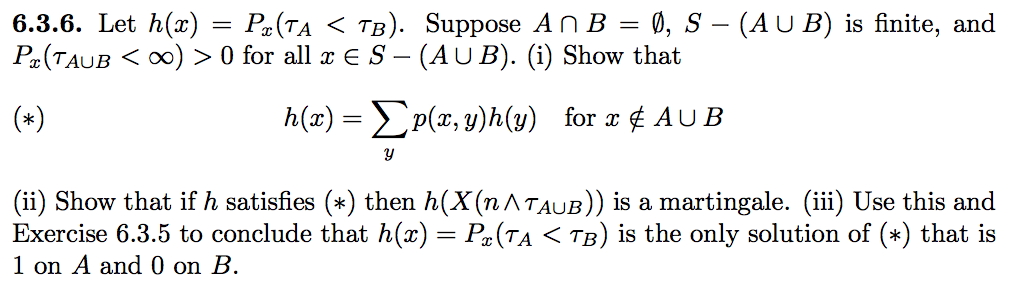
\includegraphics[width=0.7\textwidth]{d-6-3-6.png}
\end{figure}
\end{question}
\begin{solution} \hfill \\
\textbf{(i)}
Let $x \in S \setminus (A \cup B)$. Then,
\eQb
1_{\{\tau_A < \tau_B\}} &=& 1_{ \{ \tau_A < \tau_B \}} \circ \theta_1.
\eQe
It follows that
\eQnb
h(x) &=& P_x(\tau_A < \tau_B) = E_x(1_{\{\tau_A < \tau_B\}}) = 
E_x(1_{\{\tau_A < \tau_B \}} \circ \theta_1) \nonumber \\
&=& E_x(E_x(1_{\{\tau_A < \tau_B \}} \circ \theta_1 | \mathscr{F}_1)) = 
E_x(E_{X_1}(1_{\{ \tau_A < \tau_B \}})) \label{eq:6.3.6.1} \\
&=& \sum_{y} P(X_1 = y)P_y( \tau_A < \tau_B) = \sum_{y} p(x,y) P_y(\tau_A < \tau_B) 
\nonumber  
\eQne
where~\eqref{eq:6.3.6.1} holds by Markov property. 

\bigskip

\textbf{(ii)}


\bigskip


\textbf{(iii)} 

\end{solution}

\newpage


\begin{question}[6.3.7]
\hfill
\begin{figure}[h!]
  \centering
    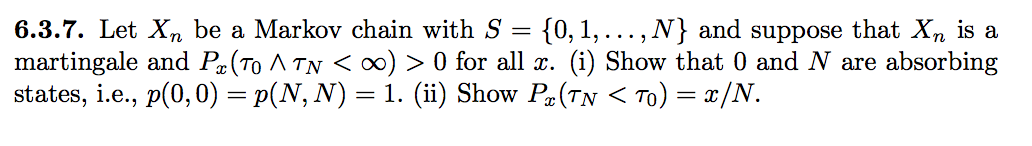
\includegraphics[width=0.7\textwidth]{d-6-3-7.png}
\end{figure}
\end{question}
\begin{solution} \hfill \\
\end{solution}

\newpage

\begin{question}[6.4.1]
\hfill
\begin{figure}[h!]
  \centering
    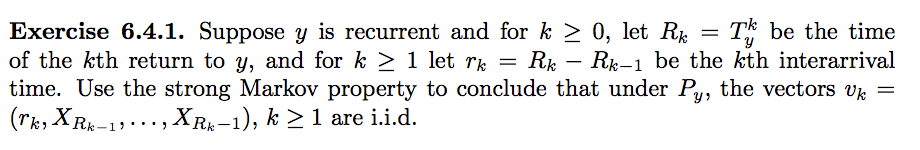
\includegraphics[width=0.7\textwidth]{d-6-4-1.png}
\end{figure}
\end{question}
\begin{solution} \hfill \\
We wish to show that
for all $k,l \in \mathbb{N}$
\end{solution}

\newpage

\begin{question}[6.4.2]
\hfill
\begin{figure}[h!]
  \centering
    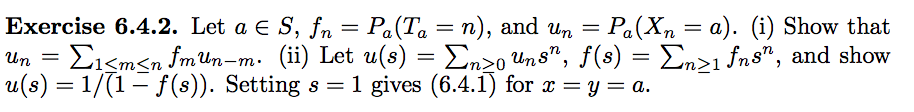
\includegraphics[width=0.7\textwidth]{d-6-4-2.png}
\end{figure}
\end{question}
\begin{solution} \hfill \\
\end{solution}

\newpage

\begin{question}[6.4.3]
\hfill
\begin{figure}[h!]
  \centering
    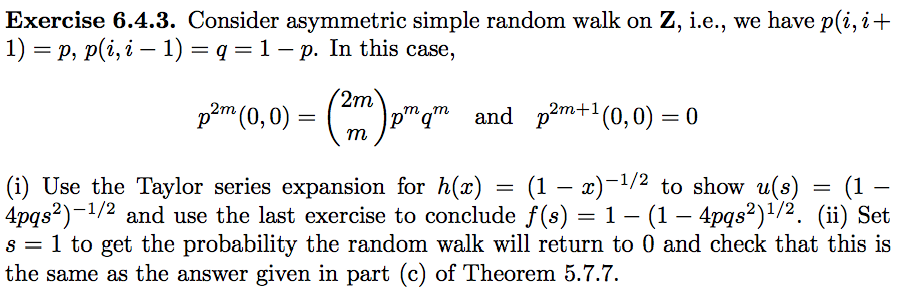
\includegraphics[width=0.7\textwidth]{d-6-4-3.png}
\end{figure}
\end{question}
\begin{solution} \hfill \\
\end{solution}

\newpage

\begin{question}[6.4.4]
\hfill
\begin{figure}[h!]
  \centering
    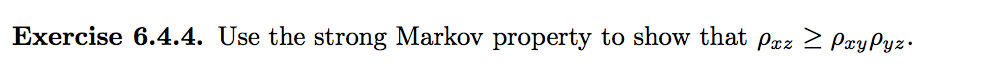
\includegraphics[width=0.7\textwidth]{d-6-4-4.png}
\end{figure}
\end{question}
\begin{solution} \hfill \\
The key insight in this problem is that if you shift the chain by a stopping time
of one state variable, then the probability of the chain 
coming back to another fixed state variable decreases. 
This relation allows one to estimate $p_{xz}$ from below
using strong Markov, which in our context is proven for a sequence space(discrete time)
of a polish state space, using Monotone class theorem.  
Recall that to define a shift operator, indexed by $\infty$,
by convention, we set
\eQb
\theta_{\infty}(w) = \triangle
\eQe
where $\triangle$ is the cemetery sample point we add to $S^{\mathbb{N}}$,
for all $w \in S^{\mathbb{N}}$. Therefore, to extend the domain of $T_z = 
\inf\{n \geq 1: X_n = z \}$ for any $z \in S$,
to include $\triangle$, if necessary, we define
\eQb
T_z(\triangle) = \infty \>\>\> \text{so} \>\>\> 1_{\{T_z < \infty\}}(\triangle) = 0,
\eQe 
With this convention.
\eQb
\{w \in S^{\mathbb{N}} : 1_{\{T_z < \infty\}} \circ \theta_{T_y}(w) = 1 \} &=& 
\{w \in S^{\mathbb{N}} : 
T_y(w) = n \text{ for some } n \geq 1 \>\>\> \\
&& \text{and} \>\>\> T_z^{n}(w) = 
\inf\{k \geq n : X_k = z\} < \infty \} \\
&=& \bigcup_{n=1}^{\infty} \{T_y = n \>\> ; \>\> T_{z}^{n} < \infty \} \\
&\subset& \bigcup_{n=1}^{\infty} \{T_z^{n} < \infty\} = \{ T_z < \infty \} 
\eQe
for any $z,y \in S$. 

\bigskip


\noindent 
Now, let $x,y,z \in S$. Then,
\eQnb
p_{xz} &=& P_x(T_z < \infty) = E_x( 1_{\{T_z < \infty\}}) 
\geq E_x( 1_{\{T_z < \infty\}} \circ \theta_{T_y}) \nonumber \\
&=& E_x( E_x(1_{\{T_z < \infty\}} \circ \theta_{T_y} |\mathscr{F}_{T_y}); T_y < \infty)
\label{eq:6.4.4.1} \\
&=& E_x( E_{X_{T_y}}(1_{\{ T_z < \infty \}} ; T_y < \infty) 
= E_x( E_{X_y}(1_{\{T_z < \infty \}} ; T_y < \infty) \label{eq:6.4.4.2} \\ 
&=& E_x( P_y( T_z < \infty) ; T_y < \infty) = P_y( T_z < \infty) P_x(T_y < \infty)
= p_{xy} p_{yz} \nonumber 
\eQne
where~\eqref{eq:6.4.4.1} holds by definition of conditional expectation, 
and~\eqref{eq:6.4.4.2} holds by strong Markov. \hfill $\qed$

\end{solution}

\newpage

\section{Chapter 2: Law of Large Numbers}

\newpage

\section{Chapter 4: Random Walks}

\begin{question}[4.1.1]
\hfill
\begin{figure}[h!]
  \centering
    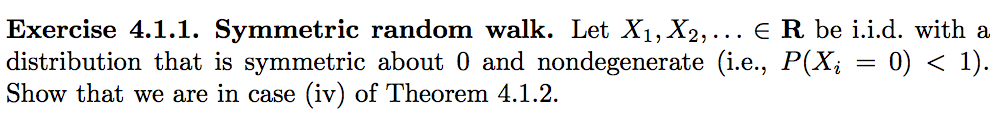
\includegraphics[width=0.7\textwidth]{d-4-1-1.png}
\end{figure}
\end{question}

\newpage

\begin{question}[4.1.2]
\hfill
\begin{figure}[h!]
  \centering
    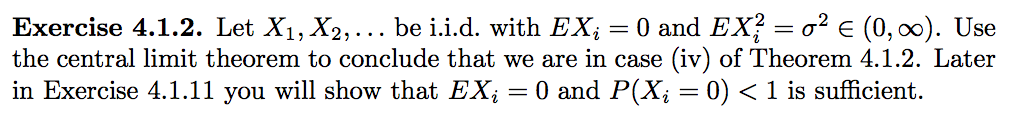
\includegraphics[width=0.7\textwidth]{d-4-1-2.png}
\end{figure}
\end{question}

\newpage

\begin{question}[4.1.3]
\hfill
\begin{figure}[h!]
  \centering
    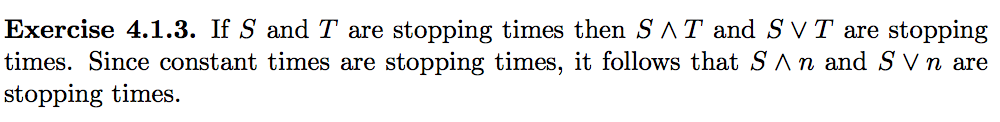
\includegraphics[width=0.7\textwidth]{d-4-1-3.png}
\end{figure}
\end{question}

\newpage

\begin{question}[4.1.4]
\hfill
\begin{figure}[h!]
  \centering
    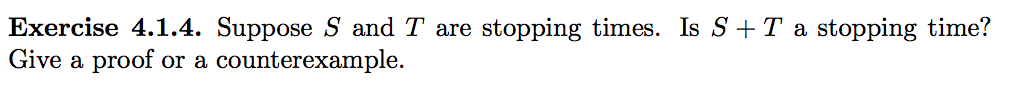
\includegraphics[width=0.7\textwidth]{d-4-1-4.png}
\end{figure}
\end{question}

\newpage

\begin{question}[4.1.5]
\hfill
\begin{figure}[h!]
  \centering
    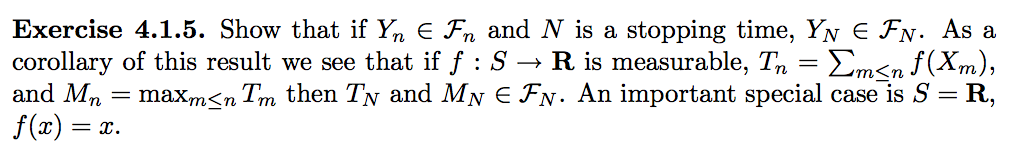
\includegraphics[width=0.7\textwidth]{d-4-1-5.png}
\end{figure}
\end{question}

\newpage

\section{Chapter 5: Martingales}

\begin{question}[5.2.1]
\hfill
\begin{figure}[h!]
  \centering
    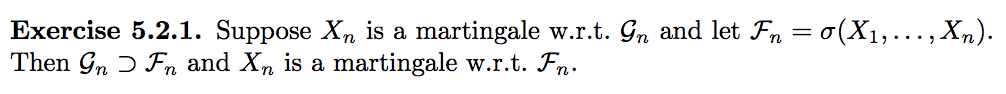
\includegraphics[width=0.7\textwidth]{d-5-2-1.png}
\end{figure}
\end{question}
\begin{solution} \hfill \\
Various properties of conditional expectations are used.

\bigskip

We compute
\eQnb
E[X_{n+1}| \mathscr{F}_n] &=& E[X_{n+1} | \mathscr{G}_{n} | 
\mathscr{F}_n] \label{eq:5.2.1.1} \\
&=& E [X_n| \mathscr{F}_n] \label{eq:5.2.1.2} \\ 
&=& X_n \label{eq:5.2.1.3}  
\eQne
for all $n \in \mathbb{N}$, where~\eqref{eq:5.2.1.1} holds by 
the Tower property,~\eqref{eq:5.2.1.2} holds by Martingale property of $\{G_n\}$
and~\eqref{eq:5.2.1.3} holds by measurability of $X_n$ w.r.t $\mathscr{F}_n$ for 
all $n \in \mathbb{N}$.  \hfill $\qed$
\end{solution}

\newpage

\begin{question}[5.2.2]
\hfill
\begin{figure}[h!]
  \centering
    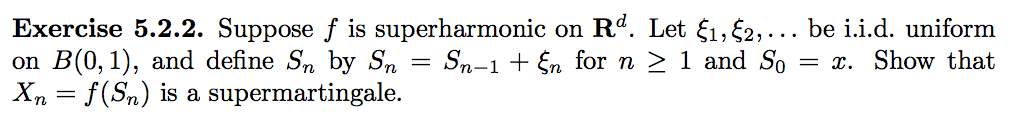
\includegraphics[width=0.7\textwidth]{d-5-2-2.png}
\end{figure}
\end{question}
\begin{solution} \hfill \\
\end{solution}

\newpage

\begin{question}[5.2.3]
\hfill
\begin{figure}[h!]
  \centering
    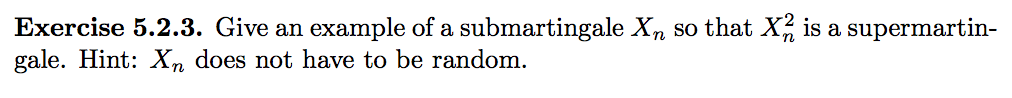
\includegraphics[width=0.7\textwidth]{d-5-2-3.png}
\end{figure}
\end{question}
\begin{solution} \hfill \\
Consider $\{X_n = 0\}$. Then, $\{X_n^2 = 0\}$, so both are processes are martingales, 
we have the desired example. \hfill $\qed$
\end{solution}

\newpage

\begin{question}[5.2.4]
\hfill
\begin{figure}[h!]
  \centering
    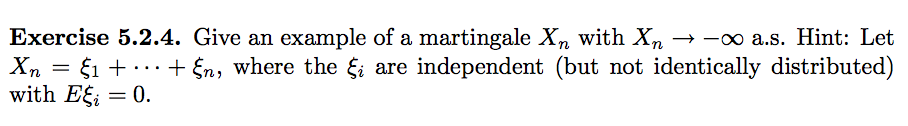
\includegraphics[width=0.7\textwidth]{d-5-2-4.png}
\end{figure}
\end{question}
\begin{solution} \hfill \\
Set $\xi_n = -1$ with probability $2^{-1}$ and $\xi_n = 2^{n}$ with probability
$2^{-(n+1)}$ 
for each $n \in \mathbb{N}$, such that they are independent. Then, by construction, 
\eQb
E[X_{n+1}| \mathscr{F}_n] &=& E[\xi_{n+1}] + E[X_n|\mathscr{F}_n] = X_n
\eQe
for all $n \in \mathbb{N}$, so $\{X_n\}$ is a martingale. Now, as
\eQb
\sum_{n=1}^{\infty} P(\xi_n \leq -1) = \infty
\eQe
by Borel-Cantelli II,
\eQb
P(\xi_n \leq -1 \>\>\> \text{i.o} ) = 1 \>\>\> \text{and} \>\>\> P(X_n \to -\infty) = 1,
\eQe
as required. \hfill $\qed$
\end{solution}

\newpage

\begin{question}[5.2.5]
\hfill
\begin{figure}[h!]
  \centering
    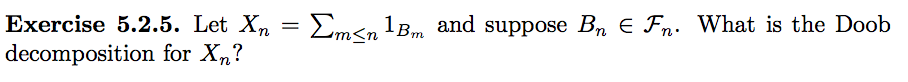
\includegraphics[width=0.7\textwidth]{d-5-2-5.png}
\end{figure}
\end{question}
\begin{solution} \hfill \\
\end{solution}

\newpage

\begin{question}[5.2.6]
\hfill
\begin{figure}[h!]
  \centering
    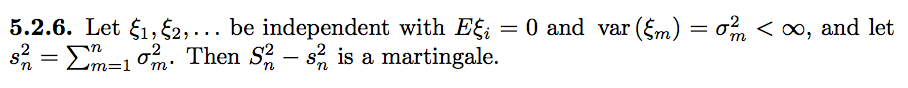
\includegraphics[width=0.7\textwidth]{d-5-2-6.png}
\end{figure}
\end{question}
\begin{solution} \hfill \\
We compute
\eQnb
E(S_{n+1}^2 - s_{n+1}^2 | \mathscr{F}_n) &=& 
E(S_n^2 | \mathscr{F}_n) + E(\xi_{n+1}^2 | \mathscr{F}_n) 
+ 2E(\xi_{n+1} S_n | \mathscr{F}_n) - s_{n+1}^2 \\
&=& S_n^2 + E(\xi_{n+1}^2) +  
\eQne
\end{solution}

\newpage

\begin{question}[5.2.7]
\hfill
\begin{figure}[h!]
  \centering
    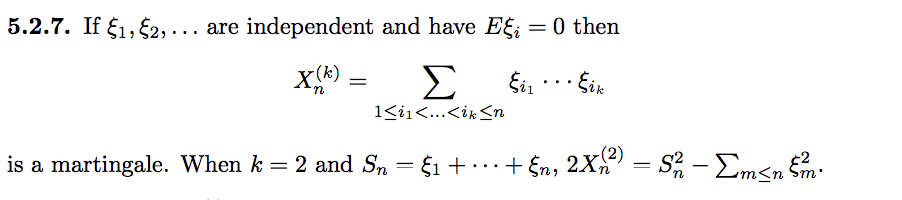
\includegraphics[width=0.7\textwidth]{d-5-2-7.png}
\end{figure}
\end{question}
\begin{solution} \hfill \\
Observe that
\eQb
1 + y \leq e^{y}
\eQe
and hence
\eQb
log(1+y) \leq y 
\eQe
for all $y \in \mathbb{R}$. Now, fix $|y| \leq 2^{-1}$. Then,
\eQb
\log(1+y) &=& \sum_{n=1}^{\infty} (-1)^{n-1} \dfrac{y^n}{n}. \\
&\geq& y - |\sum_{n=2}^{\infty} (-1)^{n-1} \dfrac{y^n}{n}| \\
&\leq& y - \dfrac{y^2}{2} (\sum_{n=1}^{\infty} \dfrac{1}{2^{n-1}}) = y + y^2. 
\eQe 
Therefore,
\eQb
|y| \leq 2^{-1} &\implies& y - y^2 \leq(1+y) 
\eQe

\end{solution}

\newpage

\begin{question}[5.2.8]
\hfill
\begin{figure}[h!]
  \centering
    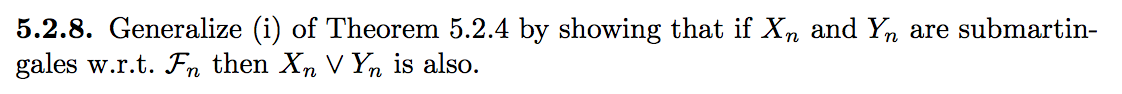
\includegraphics[width=0.7\textwidth]{d-5-2-8.png}
\end{figure}
\end{question}
\begin{solution} \hfill \\
\end{solution}

\newpage

\begin{question}[5.2.9]
\hfill
\begin{figure}[h!]
  \centering
    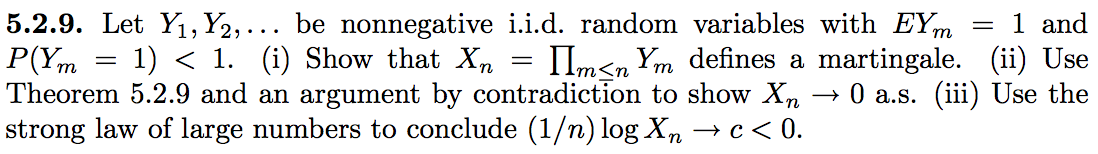
\includegraphics[width=0.7\textwidth]{d-5-2-9.png}
\end{figure}
\end{question}
\begin{solution} \hfill \\
\textbf{(i)}
As $\{Y_n\}$ are non-negative and independent, 
\eQnb
E(|X_{n}|) &=& E(|\prod_{m \leq n} Y_n|) = E(\prod_{m \leq n} Y_m) = 
\prod_{m \leq n} E(Y_m) = 1 \label{eq:5.2.9.1}
\eQne
for all $n \in \mathbb{N}$. Therefore, 
\eQnb
E(X_{n+1} | \mathscr{F}_n ) &=& E(\prod_{m \leq n+1} Y_n | \mathscr{F}_n) = 
X_{n}E(\prod_{m \leq n} Y_{n+1} | \mathscr{F}_n) \label{eq:5.2.9.2} \\
&=& X_n E(Y_{n+1}) = X_n \label{eq:5.2.9.3}  
\eQne
for all $n \in \mathbb{N}$, where~\eqref{eq:5.2.9.2} holds by theorem 5.1.7, 
and~\eqref{eq:5.2.9.1}, and~\eqref{eq:5.2.9.3} holds by independence. Therefore,
$\{X_n\}$ is a martingale. We remark that since $\{X_n\}$ is a non-negative 
martingale, it converges almost surely to
some $X_{\infty} \in L^1$ by Martingale convergence theorem. 

\bigskip

\noindent \textbf{(ii)} 
Fix $n \in \mathbb{N}$. Suppose there does not exists $\epsilon > 0$ such that
\eQb
P(|Y_n - 1| > \epsilon) > 0.
\eQe
Then, by continuity of probability,
\eQb
P(Y_ n = 1) &=& P(|Y_n - 1| = 0) = P(\bigcap_{k=1}^{\infty} |Y_n - 1| \leq k^{-1})
= \lim_{k \to \infty} P(|Y_n - 1| \leq k^{-1}) = 1, 
\eQe
which contradicts that $P(Y_n = 1 ) < 1$. Hence, as $Y_n$ is identically distributed,
we can choose $\epsilon > 0$, such that
\eQb
P(|Y_n - 1| > \epsilon) > 0
\eQe 
for all $n \in \mathbb{N}$. Now,
\eQnb
P(|X_{n+1} - X_n| \geq \epsilon \delta ) &=& P(X_n|Y_{n+1} - 1| \geq \epsilon \delta) 
\nonumber \\
&\geq& P(X_n  \geq \delta ; |Y_{n+1} - 1| > \epsilon) 
P(X_n \geq \delta)P(|Y_{n+1} - 1| > \epsilon) \label{eq:5.2.9.4} 
\eQne
for any $\delta > 0$, where~\eqref{eq:5.2.9.4} holds by independence. As $X_n$
converges almost surely,
\eQb
\lim_{n \to \infty} P(|X_{n+1} - X_n| \geq \epsilon \delta) = 0 
\eQe
and hence, by~\eqref{eq:5.2.9.4},
\eQb
\lim_{n \to \infty}P(X_n \geq \delta) = 0
\eQe
for all $\delta > 0$. Therefore, $X_n \to_{p} 0$. Since, we have
$X_n \to X_{\infty}$ almost surely, which implies $X_n \to_{p} X_{\infty}$, we have
$X_{\infty} = 0$ almost surely, and $X_n \to 0$ almost surely.

\bigskip

\noindent \textbf{(iii)} 
 
\end{solution}

\newpage

\begin{question}[5.2.10]
\hfill
\begin{figure}[h!]
  \centering
    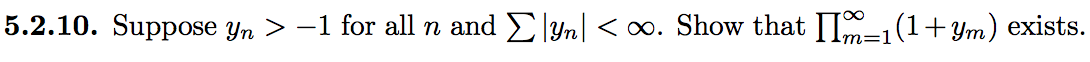
\includegraphics[width=0.7\textwidth]{d-5-2-10.png}
\end{figure}
\end{question}
\begin{solution} \hfill \\
The key idea in this problem is that one can make a use of Taylor estimates of
exponential and log, to prove convergence of a product($x \mapsto x^2$ is is below
$x \mapsto x$ for any $|x| \leq 1$!). 

\bigskip

\noindent Observe that
\eQb
1 + y \leq e^{y}
\eQe
and hence
\eQb
\log(1+y) \leq y 
\eQe
for all $y > -1$. Now, fix $|y| \leq 2^{-1}$. Then,
\eQb
\log(1+y) &=& y - \dfrac{y^2}{2} + \dfrac{y^3}{3} + \cdot\cdot\cdot  \\
&\geq& y - \left|-\dfrac{y^2}{2} + \dfrac{y^3}{3} + \cdot\cdot\cdot \right|  \\
&\geq& y - \dfrac{y^2}{2} \left|1 + \dfrac{1}{2} + \cdot\cdot\cdot  \right| = y - y^2 \\
\eQe 
Therefore,
\eQb
|y| \leq 2^{-1} &\implies& y - y^2 \leq \log(1+y) \leq y.
\eQe
Now, as $\sum_{n=1}^{\infty} |y_n| < \infty$, we can choose $M$ large enough such that
\eQnb
|y_n| &\leq& 2^{-1} \label{eq:5.2.10.1}  
\eQne
for all $n \geq M$. Since $\sum_{n=1}^{\infty} |y_n| < \infty$ and~\eqref{eq:5.2.10.1},
$\sum_{n=M}^{\infty} y_n$ and $\sum_{n=M}^{\infty} y_n^2$ converge, and hence
$\sum_{n=M}^{\infty} y_n - y_n^2$ converges. By comparison,
\eQb
\sum_{n=k}^{\infty} y_n - y_n^2 \leq \sum_{n = k}^{\infty} \log(1 + y_n) 
\leq \sum_{n=k}^{\infty} y_n
\eQe 
for all $k \geq M$. Letting $k \to \infty$,
\eQb
\sum_{n=k}^{\infty} \log(1+y_n) \to 0 
\eQe
and hence
\eQb
\sum_{n=1}^{m} \log(1+y_n) = \log(\prod_{n=1}^{m}(1+y_n))  \>\>\>  \text{converges.} 
\eQe
By continuity of $\log$, $\prod_{n=1}^{\infty}(1+y_n)$ exists. \hfill $\qed$ 

\end{solution}

\newpage

\begin{question}[5.2.11]
\hfill
\begin{figure}[h!]
  \centering
    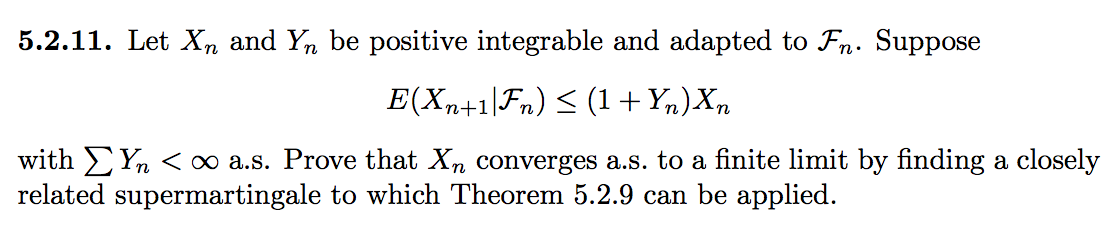
\includegraphics[width=0.7\textwidth]{d-5-2-11.png}
\end{figure}
\end{question}
\begin{solution} \hfill \\
\end{solution}

\newpage

\begin{question}[5.2.12]
\hfill
\begin{figure}[h!]
  \centering
    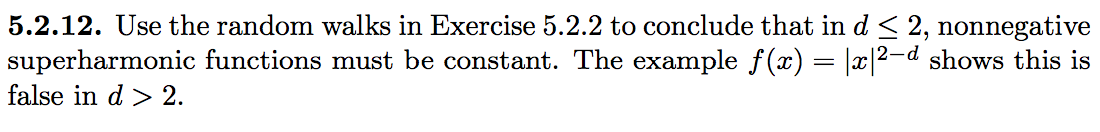
\includegraphics[width=0.7\textwidth]{d-5-2-12.png}
\end{figure}
\end{question}
\begin{solution} \hfill \\
\end{solution}

\newpage

\begin{question}[5.2.13]
\hfill
\begin{figure}[h!]
  \centering
    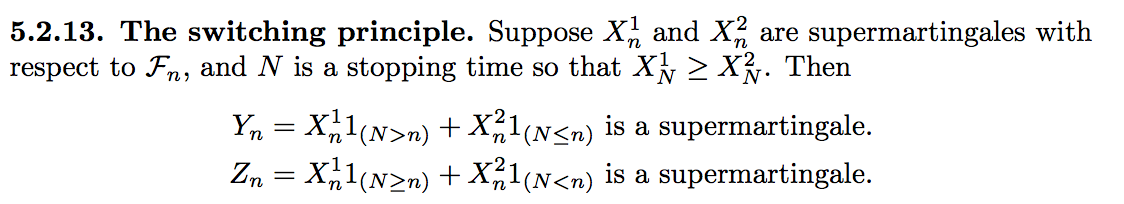
\includegraphics[width=0.7\textwidth]{d-5-2-13.png}
\end{figure}
\end{question}
\begin{solution} \hfill \\
\end{solution}
\end{document}
